% Options for packages loaded elsewhere
\PassOptionsToPackage{unicode}{hyperref}
\PassOptionsToPackage{hyphens}{url}
%
\documentclass[
  12pt,
]{article}
\usepackage{amsmath,amssymb}
\usepackage{iftex}
\ifPDFTeX
  \usepackage[T1]{fontenc}
  \usepackage[utf8]{inputenc}
  \usepackage{textcomp} % provide euro and other symbols
\else % if luatex or xetex
  \usepackage{unicode-math} % this also loads fontspec
  \defaultfontfeatures{Scale=MatchLowercase}
  \defaultfontfeatures[\rmfamily]{Ligatures=TeX,Scale=1}
\fi
\usepackage{lmodern}
\ifPDFTeX\else
  % xetex/luatex font selection
\fi
% Use upquote if available, for straight quotes in verbatim environments
\IfFileExists{upquote.sty}{\usepackage{upquote}}{}
\IfFileExists{microtype.sty}{% use microtype if available
  \usepackage[]{microtype}
  \UseMicrotypeSet[protrusion]{basicmath} % disable protrusion for tt fonts
}{}
\makeatletter
\@ifundefined{KOMAClassName}{% if non-KOMA class
  \IfFileExists{parskip.sty}{%
    \usepackage{parskip}
  }{% else
    \setlength{\parindent}{0pt}
    \setlength{\parskip}{6pt plus 2pt minus 1pt}}
}{% if KOMA class
  \KOMAoptions{parskip=half}}
\makeatother
\usepackage{xcolor}
\usepackage[margin=1in]{geometry}
\usepackage{longtable,booktabs,array}
\usepackage{calc} % for calculating minipage widths
% Correct order of tables after \paragraph or \subparagraph
\usepackage{etoolbox}
\makeatletter
\patchcmd\longtable{\par}{\if@noskipsec\mbox{}\fi\par}{}{}
\makeatother
% Allow footnotes in longtable head/foot
\IfFileExists{footnotehyper.sty}{\usepackage{footnotehyper}}{\usepackage{footnote}}
\makesavenoteenv{longtable}
\usepackage{graphicx}
\makeatletter
\def\maxwidth{\ifdim\Gin@nat@width>\linewidth\linewidth\else\Gin@nat@width\fi}
\def\maxheight{\ifdim\Gin@nat@height>\textheight\textheight\else\Gin@nat@height\fi}
\makeatother
% Scale images if necessary, so that they will not overflow the page
% margins by default, and it is still possible to overwrite the defaults
% using explicit options in \includegraphics[width, height, ...]{}
\setkeys{Gin}{width=\maxwidth,height=\maxheight,keepaspectratio}
% Set default figure placement to htbp
\makeatletter
\def\fps@figure{htbp}
\makeatother
\setlength{\emergencystretch}{3em} % prevent overfull lines
\providecommand{\tightlist}{%
  \setlength{\itemsep}{0pt}\setlength{\parskip}{0pt}}
\setcounter{secnumdepth}{5}
% definitions for citeproc citations
\NewDocumentCommand\citeproctext{}{}
\NewDocumentCommand\citeproc{mm}{%
  \begingroup\def\citeproctext{#2}\cite{#1}\endgroup}
\makeatletter
 % allow citations to break across lines
 \let\@cite@ofmt\@firstofone
 % avoid brackets around text for \cite:
 \def\@biblabel#1{}
 \def\@cite#1#2{{#1\if@tempswa , #2\fi}}
\makeatother
\newlength{\cslhangindent}
\setlength{\cslhangindent}{1.5em}
\newlength{\csllabelwidth}
\setlength{\csllabelwidth}{3em}
\newenvironment{CSLReferences}[2] % #1 hanging-indent, #2 entry-spacing
 {\begin{list}{}{%
  \setlength{\itemindent}{0pt}
  \setlength{\leftmargin}{0pt}
  \setlength{\parsep}{0pt}
  % turn on hanging indent if param 1 is 1
  \ifodd #1
   \setlength{\leftmargin}{\cslhangindent}
   \setlength{\itemindent}{-1\cslhangindent}
  \fi
  % set entry spacing
  \setlength{\itemsep}{#2\baselineskip}}}
 {\end{list}}
\usepackage{calc}
\newcommand{\CSLBlock}[1]{\hfill\break\parbox[t]{\linewidth}{\strut\ignorespaces#1\strut}}
\newcommand{\CSLLeftMargin}[1]{\parbox[t]{\csllabelwidth}{\strut#1\strut}}
\newcommand{\CSLRightInline}[1]{\parbox[t]{\linewidth - \csllabelwidth}{\strut#1\strut}}
\newcommand{\CSLIndent}[1]{\hspace{\cslhangindent}#1}
\usepackage{setspace} \usepackage{lineno} \usepackage{placeins} \usepackage[nottoc,notlof,notlot]{tocbibind} \renewcommand{\contentsname}{} \renewcommand{\listfigurename}{} \renewcommand{\listtablename}{} \usepackage{sectsty} \sectionfont{\centering}
\ifLuaTeX
  \usepackage{selnolig}  % disable illegal ligatures
\fi
\usepackage{bookmark}
\IfFileExists{xurl.sty}{\usepackage{xurl}}{} % add URL line breaks if available
\urlstyle{same}
\hypersetup{
  hidelinks,
  pdfcreator={LaTeX via pandoc}}

\author{}
\date{\vspace{-2.5em}}

\begin{document}

\doublespacing

\begin{center}
    
\textbf{\Large Applying effective environmental forecasts to Management Strategy Evaluation of yellowtail flounder}
    
\textsc{Sophie Wulfing$^{1*}$ Chengxue Li$^{3}$ Scott I. Large$^{2}$ Vincent Saba$^{2}$ Gavin Fay$^{1}$\\}
\vspace{3 mm}
\normalsize{\indent $^1$School for Marine Science and Technology, University of Massachusetts Dartmouth, New Bedford, MA, 02747, USA\\ $^2$NOAA, National Marine Fisheries Service, Woods Hole, MA 02543, USA\\ $^3$School of Marine and Atmospheric Sciences, Stony Brook University, Stony Brook, NY 11794, USA\\}
$\text{*}$ Corresponding authors: Sophie Wulfing (SophieWulfing@gmail.com)
\end{center}

\newpage

\linenumbers

\section{ABSTRACT}\label{abstract}

The US Northeast Continental shelf is the fastest warming marine ecosystem in the United States and understanding this change is imperative to maintaining the sustainability and productivity of this region's fishery. Management Strategy Evaluation (MSE) is a technique in fisheries management to simulate and compare the likely outcomes of different management actions, assess trade-offs of different management options, and has been used to create more climate-ready management plans. However, predicting future environmental covariates such as bottom temperature can be challenging, as these conditions are subject to high stochasticity. In this study, we analyze the different choices made when projecting or forecasting future environmental conditions within assessments, what subsequent catch advice is generated from the MSE, and how this affects long-term fishery dynamics. We use the Georges Bank Yellowtail Flounder (\emph{Limanda ferruginea}) as it is an important stock to the Northeast groundfish fishery and its recruitment has been shown to be impacted by bottom ocean temperatures. Results focusing on recruitment-environment relationships have shown that using a 5 year temperature average to project forward in the management period most accurately estimates `true' environmental covariates. However, among different projection decisions, including integrating environmental forecasts of varying accuracy, there is a limited impact on the model performance and output, and the model is more influenced by changes to recruitment variability and assessment frequency.

\section{INTRODUCTION}\label{introduction}

As the world's oceans are complex physical and chemical systems, climate change has impacted oceans in a variety of ways such as increased water temperature and acidification, and changes in ocean currents (Fabry et al., 2008; Guinotte \& Fabry, 2008; Abraham et al., 2013; Sydeman et al., 2015; Wilson et al., 2016; Poloczanska et al., 2016; García Molinos et al., 2017; Friedland et al., 2022; Cheng et al., 2024). As a result, different marine species are projected to have complex and varying responses to these environmental shifts depending on species' life histories, thermal tolerances, mobility, and other aspects of the species' biology (Guinotte \& Fabry, 2008; Chown et al., 2010; Hönisch et al., 2012; Punt et al., 2014; Stewart et al., 2014; Sydeman et al., 2015; Poloczanska et al., 2016; Wilson et al., 2016; Chaikin et al., 2024). This creates compounding challenges when managing commercially-important fisheries. Fish stocks have already been shown to alter food chain interactions as well as increase fishing effort by changing distributions away from traditional fishing grounds or changing the time of year in which they visit these areas (Overholtz et al., 2011; Albouy et al., 2014; Stewart et al., 2014; Sydeman et al., 2015; Poloczanska et al., 2016; Wilson et al., 2016; García Molinos et al., 2017; Tommasi et al., 2017a; Fulton, 2021; Chaikin et al., 2024).

The US Northeast continental shelf has warmed faster than any other marine ecosystem in the United States (V. S. Saba et al., 2016; Kleisner et al., 2017; V. Saba et al., 2023b). The varying responses to climate change across fished species has presented challenges in accurately assessing stock health of various species in the region, however these environmental covariates have rarely been incorporated into stock assessments in the Northeast U.S. (Hare et al., 2016; Kleisner et al., 2017; Mazur et al., 2023a). These covariates have been shown to reduce retrospective patterns and increase projection accuracy in New England stocks of species including Atlantic Cod, haddock, yellowtail flounder, and winter flounder (Buckley et al., 2004; Klein et al., 2017). However, incorporating environmental covariates into stock assessments is difficult and a very clear and strong relationship between environmental change and population dynamics must be shown or else improper use of an environmental covariate could lead to poorer rather than better estimation performance (Haltuch \& Punt, 2011; Punt et al., 2014; Ehrlén \& Morris, 2015; Britten et al., 2024; Miller et al., 2023).

The current structure of management in the United States includes periodic, scheduled evaluations of stock status and subsequent management advice called Management Track Assessments (MTAs) (\textbf{fisheriesManagementTrackStock2026?}). Here, managers must take current data regarding the stock's health and make decisions for the next several years regarding catch advice and management measures. This means that the assessment and predictions of stock health must hold up over several years until the next MTA. Therefore, managers must make multiple decisions regarding predicted stock-recruit relationships, mortality, and how to consider environmental and population uncertainty in these assessment models. The incorporation of environmental covariates has been shown to decrease this uncertainty in management predictions across many stocks worldwide (Hollowed et al., 2011a; Wayte, 2013; Punt et al., 2014; Tommasi et al., 2017b; Stram \& Holsman, 2022; Mazur et al., 2023b; V. Saba et al., 2023a). However, decisions on how exactly to project environmental conditions between MTAs are important to consider when predicting stock dynamics. With recent improvements, ocean dynamic models are able to offer improved predictions of future stock dynamics and are being used in stocks worldwide. However, the spatial and temporal scale of these models is relevant (Hobday et al., 2016). Future climate is also difficult to estimate as there is a lot of uncertainty and climate change is a very chaotic process (Punt et al., 2014). As assessments attempt to capture future population trends, forecasting environmental trends is also imperative, however this can be challenging as optimal decisions can change depending on scale, species, and which environmental covariates are used (Kell et al., 2005; Hollowed et al., 2011b; Tommasi et al., 2017a; Stram \& Holsman, 2022). In a simulation-estimation experiment, Britten et al. (2024) found that there was no discernable difference in stock dynamics if ocean temperature was predicted using a self-updating average called a first-order Auto Regressive (AR(1)) model or if the temperature was predicted using the mean of the last five years. Further, Kell et al. (2005) showed that climate change has a limited effect in the short term for Atlantic cod, and only long term simulations showed an effect on stock dynamics and recovery. Northeast Fisheries Science Center, Woods Hole, MA, USA et al. (2025) used both recent averages and AR(1) estimations of future climate to predict that Georges Bank yellowtail flounder stocks could recover under certain climate conditions, but the efficacy and catch advice of each projection was not compared. This project aims to build off of these findings. Here, we expand the types of projections that have been tested by previous research, simulate over a greater number of years than what other similar studies have, and assess how catch advice and fishery dynamics may respond to changing projections.

Management Strategy Evaluations (MSEs) are decision making frameworks that allow assessors to simulate and compare the sustainability and tradeoffs associated with different management decisions (Hollowed et al., 2011b; Tommasi et al., 2017a; Mazur et al., 2023a; V. Saba et al., 2023b). As a state-space framework, MSEs use feedback loops between the Operating Model (OM), which simulates the `real-world' fishery dynamics such as stock recruitment, growth, natural mortality, and fishing mortality, and the Estimation Model (EM), which simulates a management assessment. The EM essentially `samples' the OM to come up with its own estimations of stock status, predicted fishing mortality, and gives subsequent catch advice based on the estimated health of the real world system in the OM (Bunnefeld et al., 2011; Punt et al., 2016a). This is intended to replicate real-world stock assessments, which are imperfect representations of real-world dynamics and set catch advice for several years in advance. Applying climate change covariates and MSE to New England groundfish has shown to improve the robustness of stock assessments (Mazur et al., 2023a). Populations' responses to climate change can be complex, as fish exhibit different sensitivities to environmental conditions depending on their lifestage, and different environmental changes (i.e.~increased sea surface or bottom temperature, changes in salinity, and altered currents) will have different effects on populations (Hollowed et al., 2011b). Further in 2025, the Northeast Region Coordinating Council (NRCC) reduced the frequency of management stock assessments from three-year cycles to five-year cycles due to decreased resources and capacity ({``Current {Stock Assessment Schedules},''} 2026), which could further influence how climate should be considered in these assessments. As fisheries change in response to these altered dynamics, the need for climate-ready fisheries management is imperative (Stram \& Holsman, 2022; V. Saba et al., 2023b). The MSE framework allows for simultaneous testing of these features, while considering the pros and cons of different hypothetical measures to determine the appropriate management response to these changing conditions (Punt et al., 2016b).

The yellowtail flounder (\emph{Limanda ferruginea}) has a long history of harvest in the US Atlantic Coast. However due to stock collapse in the 1980s, it is now primarily caught as bycatch in other surrounding fisheries (CITE RTA). Yellowtail flounder is managed as three distinct stocks in the Northeast US; Southern New England, Gulf of Maine, and Georges Bank. Yellowtail flounder are sensitive to water temperatures at the larval phase (Laurence \& Howell, 1981; \textbf{xuEvaluatingUtilityGulf2018?}). The Georges Bank stock has been shown to shift its distribution northward in response to warming ocean temperatures (Murawski, 1993; Nye et al., 2009; Hyun et al., 2014). This stock has been in decline starting in the 1970s, leading to a collapse in the early 1990s (Stone et al., 2004). Recently, ocean bottom temperature has been shown to have a strong link to the recruitment of Georges Bank yellowtail flounder, and the incorporation of this environmental covariate has been shown to improve stock assessment accuracy and prediction success {[}Johnson et al. (1999); Kerr et al. (2022); CITE RESEARCH TRACK{]}. Because this relationship between environment and stock dynamics has a clear linkage, inclusion of environmental covariates have improved assessment success, and this stock has a long history of data collection, we use Georges Bank yellowtail flounder as a case study. We aim to incorporate bottom temperature into stock assessments and the MSE framework in order to assess different choices when projecting bottom temperature, how this affects forecasts in assessments, and subsequent tactical fishery management advice of Georges Bank yellowtail flounder.

\section{METHODS}\label{methods}

\subsection{Operating Model Development and Conditioning}\label{operating-model-development-and-conditioning}

Operating models were conditioned on the current assessment for the Georges Bank yellowtail flounder (CITE ASSESSMENT, SUPPLEMENTAL MATERIAL). Operating models, estimation models, and all simulation testing was conducted using the R package whamMSE (Li, 2025). As per the model parameterization in yellowtail stock assessment, process error was included in the process error is included in the NAA estimates. 100 simulations were run with each experiment, allowing for different realizations of various possible fishery dynamics. As the data used to condition the OM spanned from 1973 to 2022, this was considered the hindcast period and model dynamics were projected until 2072 to test a 50 year projection period.

For the environmental covariate of bottom temperature, we used a dataset developed by Du Pontavice et al. (2023), which is also used in the Georges Bank yellowtail flounder stock assessment CITE ASSESSMENT. We projected the `real-world' temperature in the OM by conducting a linear regression on the existing data points and then projecting future temperatures along this trendline with added variation around a normal distribution. First, the Woods Hole Assessment Model was fitted to real Yellowtail flounder data from the NEFSC survey to serve as the basis for the OM. This base-OM was used to estimate parameters for numbers-at-age, selectivity, recruitment, and ecological covariate. These parameters were then treated as `truth' in our simulation and were used in the second OM we developed for the projections. This second OM, with all of the parameters already estimated, fixes the environmental covariate at a true state with no process error, however observation error is still included. This allowed us to run the 100 simulations of various temperature projections in our Estimation Model while maintaining the same `real-world' state to allow us to compare EM performances.

\subsubsection{Bias Experiment}\label{bias-experiment}

As a first experiment, we tested the consequences of using incorrect climate projections in the EM under different real world climate scenarios in the OM.

In the base-case scenario, ocean floor temperatures were projected by taking the overall trend of the hindcast data and continuing that trend forward for the 50 year projection period with added variability. In the hindcast period from 1972 to 2022, ocean floor temperatures were increasing at about 0.02 °C per year. For the base-case scenario, this trend was projected forward from 2023 to 2072 as a time-variant annual mean of a normal distribution. The temperature for any projection year was drawn from that normal distribution, using the standard deviation estimated by Du Pontavice et al. (2023) for bottom temperatures in the hindcast period.

We then considered three more climate scenarios: a low-temperature scenario where the trend of this time-variant annual mean was -0.04 (multiplying the hindcast trend by -2), a medium-low scenario where the time variant annual mean had a -0.02 (multiplying the hindcast trend by -1) change per year, and a high-temperature scenario where the time-variant annual mean was 0.04 (multiplying the hindcast trend by 2). All scenarios used the same standard deviation found from the Du Pontavice et al. (2023) hindcast period.

\subsubsection{Projection, 5-year, and Sensitivity Tests}\label{projection-5-year-and-sensitivity-tests}

In the subsequent experiments, we tested how different projection choices in the EM affect fishery dynamics in a normal yellowtail flounder assessment scenario with a three year assessment cycle, a 5 year assessment period, and an experiment using a reduced random effects on recruitment parameter of 0.2. As each EM uses a different projected temperature time series, the impact of these different temperature time series may be absorbed by the random effects on NAA, so the observable impact of different bottom temperatures may be hidden by this variation in the NAA. Reducing these random effects will give the ecological covariate a more direct impact on future dynamics, amplifying the effects of different projection choices.

\subsection{EMs}\label{ems}

The Estimation Model (EM) simulates the survey and assessment process in the fishery, including observation errors. Stock assessments were tested with the catch advice following the 0.75 Fmsy NEFMC control rule, meaning catch is limited to 75\% of what is calculated to be the maximum rate of sustainable extraction in the assessment. We tested a 50 year projection period, simulating 50 years of fishery dynamics, with the EM conducting an assessment and setting catch advice every three years.

\subsubsection{Temperature Bias in EMs}\label{temperature-bias-in-ems}

For the bias test, we used the four OM scenarios as the four `real-world' temperature trends and tested them against four EMs that were identical except for this temperature projection \ref{fig:EMTemps}. The purpose of this experiment was to assess the performance of Estimation Models using an incorrect assumption of temperature trends in assessment processes, and how these consequences change under different future climate scenarios. Each of the four OM temperature time series (low-temperature, medium-low temperature, the base case, and the high-temperature scenarios) were then tested against EMs using the same four temperature trends, simulating a low, medium-low, and high bias scenario along with the base-case temperature trend. Each combination of real world temperature trends and bias forecasts in the EM was simulated 100 times to ensure robustness of model results. Any non-converged models resulted in the elimination of that whole simulation.

\begin{figure}

\includegraphics[width=29.17in]{Biases/EMtempPlot} \caption{Temperature projections of the different Bias tests. In each test, one of these four temperture time series was used as the OM and this was tested against 4 EMs; each using one of the time series as a hypothetical assumption about temperature trends}\label{fig:EMTemps}
\end{figure}

\subsubsection{Projection EMs}\label{projection-ems}

After comparing biased projections through the MSE process, the experiment was repeated except we used only the original OM temperature projection (the one that maintains the trend from the Du Pontavice et al. (2023) data set). For the EMs, two biased projections were kept (a `bad' projection, which doubled the rate of temperature increase compared to the OM, and a `good' projection, which maintained the general trend of temperature increase with added stochasticity). The purpose of keeping these two biased time series was to compare `correct' and `incorrect' assumptions about climate with different projection choices in the Estimation Model. For the various projection choices, stock advice is given with different assumptions for how climate will change over the three-year timespan in between assessments. The process for calculating different temperature projections is shown in figure \ref{fig:EMTempsProj}, but at each assessment year, each projection choices takes into account the most recent environmental information (in this case bottom temperature) of the previous years and calculates an assumed temperature time series over the next three years (until the next stock assessment, where temperature predictions are recalculated given the most recent environmental data).

Figure \ref{fig:EMTempsProj} demonstrates the various projection options available to fisheries management. AR(1) (Auto-Regressive1) projection uses an updated mean at each timestep for the projection. The Recent Window process uses the mean of the previous 5 years in its projection. Historical average uses the average of all data points collected in the hindcase period of 1972-2022. The recent Trend process, Similar to Recent Window, takes the last 5 years of data and uses the linear regression of the last 5 years as its projection. The Terminal Year projection uses the final temperature observation across the projection period. We also included a `Good Projection' which uses the same general trend of temperature as in the OM with added stochasticity. A Bad Projection was also included. Same as the Medium-Low bias in the previous experiment, this projection tests projection with a bias significantly lower than temperatures from the OM. We also tested an EM with No Temperature time series used (not pictured in figure \ref{fig:EMTempsProj}) - This projection does not consider environmental covariates in its projection.

\subsubsection{5-year and Sensitivity EMs}\label{year-and-sensitivity-ems}

We repeated the experiment with different projection choices, but with a reduced parameter for random effects on this stocks recruitment (from 0.655 to 0.2 in recruitment and from 0.72 to 0.2 in age classes 2+) Lower variance on recruitment forces interannual variation in recruitment to respond more directly to environmental variation which could potentially amplify the consequences of different projection choices.

We also tested how changing assessment intervals would influence fishery dynamics under different projection choices, increasing the time period in between assessments from three years to every five years. This reduced management schedule is being adopted widely in the Northeast United States, so this experiment is intended to assess the performance of less frequent stock assessments under changing ocean conditions.

\begin{figure}
\centering
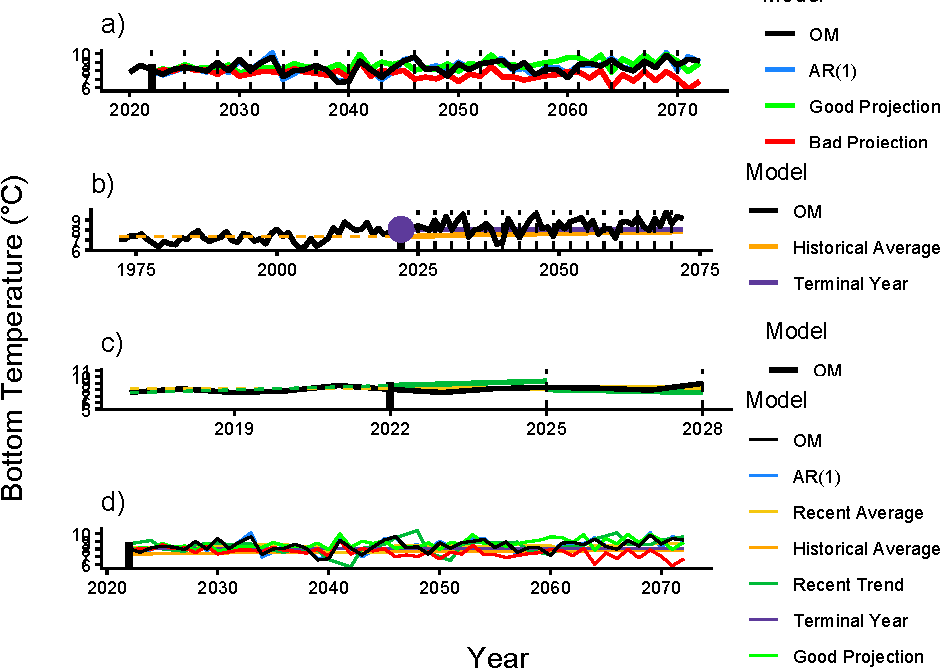
\includegraphics{YT_ProjDraft3_files/figure-latex/EMTempsProj-1.pdf}
\caption{\label{fig:EMTempsProj}Graphical representation of each porjection choice. a)}
\end{figure}

\subsection{Performance Metrics}\label{performance-metrics}

WRITE THIS

\section{RESULTS}\label{results}

\newpage

\textbf{References}

\phantomsection\label{refs}
\begin{CSLReferences}{1}{2}
\bibitem[\citeproctext]{ref-abraham2013}
Abraham, J. P., Baringer, M., Bindoff, N. L., Boyer, T., Cheng, L. J., Church, J. A., Conroy, J. L., Domingues, C. M., Fasullo, J. T., Gilson, J., Goni, G., Good, S. A., Gorman, J. M., Gouretski, V., Ishii, M., Johnson, G. C., Kizu, S., Lyman, J. M., Macdonald, A. M., \ldots{} Willis, J. K. (2013). A review of global ocean temperature observations: Implications for ocean heat content estimates and climate change. \emph{Reviews of Geophysics}, \emph{51}(3), 450--483. \url{https://doi.org/10.1002/rog.20022}

\bibitem[\citeproctext]{ref-albouy2014}
Albouy, C., Velez, L., Coll, M., Colloca, F., Le Loc'h, F., Mouillot, D., \& Gravel, D. (2014). From projected species distribution to food{-}web structure under climate change. \emph{Global Change Biology}, \emph{20}(3), 730--741. \url{https://doi.org/10.1111/gcb.12467}

\bibitem[\citeproctext]{ref-brittenIdentificationPerformanceStockrecruitment2024}
Britten, G. L., Brooks, E., \& Miller, T. (2024). \emph{Identification and performance of stock-recruitment functions in state space assessment models}. NEFSC.

\bibitem[\citeproctext]{ref-buckley2004}
Buckley, L. J., Caldarone, E. M., \& Lough, R. G. (2004). Optimum temperature and food{-}limited growth of larval Atlantic cod ( {\emph{Gadus morhua}} ) and haddock ( {\emph{Melanogrammus aeglefinus}} ) on Georges Bank. \emph{Fisheries Oceanography}, \emph{13}(2), 134--140. \url{https://doi.org/10.1046/j.1365-2419.2003.00278.x}

\bibitem[\citeproctext]{ref-bunnefeldManagementStrategyEvaluation2011}
Bunnefeld, N., Hoshino, E., \& Milner-Gulland, E. J. (2011). Management strategy evaluation: A powerful tool for conservation? \emph{Trends in Ecology \& Evolution}, \emph{26}(9), 441--447. \url{https://doi.org/10.1016/j.tree.2011.05.003}

\bibitem[\citeproctext]{ref-chaikin2024}
Chaikin, S., Riva, F., Marshall, K. E., Lessard, J.-P., \& Belmaker, J. (2024). Marine fishes experiencing high-velocity range shifts may not be climate change winners. \emph{Nature Ecology \& Evolution}, \emph{8}(5), 936--946. \url{https://doi.org/10.1038/s41559-024-02350-7}

\bibitem[\citeproctext]{ref-cheng2024}
Cheng, L., Abraham, J., Trenberth, K. E., Boyer, T., Mann, M. E., Zhu, J., Wang, F., Yu, F., Locarnini, R., Fasullo, J., Zheng, F., Li, Y., Zhang, B., Wan, L., Chen, X., Wang, D., Feng, L., Song, X., Liu, Y., \ldots{} Lu, Y. (2024). New Record Ocean Temperatures and Related Climate Indicators in 2023. \emph{Advances in Atmospheric Sciences}, \emph{41}(6), 1068--1082. \url{https://doi.org/10.1007/s00376-024-3378-5}

\bibitem[\citeproctext]{ref-chown2010}
Chown, S., Hoffmann, A., Kristensen, T., Angilletta, M., Stenseth, N., \& Pertoldi, C. (2010). Adapting to climate change: a perspective from evolutionary physiology. \emph{Climate Research}, \emph{43}(1), 3--15. \url{https://doi.org/10.3354/cr00879}

\bibitem[\citeproctext]{ref-CurrentStockAssessment2026}
Current {Stock Assessment Schedules}. (2026). In \emph{New England Fishery Management Council}.

\bibitem[\citeproctext]{ref-dupontavice2023}
Du Pontavice, H., Chen, Z., \& Saba, V. S. (2023). A high-resolution ocean bottom temperature product for the northeast U.S. continental shelf marine ecosystem. \emph{Progress in Oceanography}, \emph{210}, 102948. \url{https://doi.org/10.1016/j.pocean.2022.102948}

\bibitem[\citeproctext]{ref-ehrluxe9n2015}
Ehrlén, J., \& Morris, W. F. (2015). Predicting changes in the distribution and abundance of species under environmental change. \emph{Ecology Letters}, \emph{18}(3), 303--314. \url{https://doi.org/10.1111/ele.12410}

\bibitem[\citeproctext]{ref-fabry2008}
Fabry, V. J., Seibel, B. A., Feely, R. A., \& Orr, J. C. (2008). Impacts of ocean acidification on marine fauna and ecosystem processes. \emph{ICES Journal of Marine Science}, \emph{65}(3), 414--432. \url{https://doi.org/10.1093/icesjms/fsn048}

\bibitem[\citeproctext]{ref-friedland2022}
Friedland, K. D., Miles, T., Goode, A. G., Powell, E. N., \& Brady, D. C. (2022). The Middle Atlantic Bight Cold Pool is warming and shrinking: Indices from in situ autumn seafloor temperatures. \emph{Fisheries Oceanography}, \emph{31}(2), 217--223. \url{https://doi.org/10.1111/fog.12573}

\bibitem[\citeproctext]{ref-fulton2021}
Fulton, E. A. (2021). Opportunities to improve ecosystem{-}based fisheries management by recognizing and overcoming path dependency and cognitive bias. \emph{Fish and Fisheries}, \emph{22}(2), 428--448. \url{https://doi.org/10.1111/faf.12537}

\bibitem[\citeproctext]{ref-garcuxedamolinos2017}
García Molinos, J., Burrows, M. T., \& Poloczanska, E. S. (2017). Ocean currents modify the coupling between climate change and biogeographical shifts. \emph{Scientific Reports}, \emph{7}(1), 1332. \url{https://doi.org/10.1038/s41598-017-01309-y}

\bibitem[\citeproctext]{ref-guinotte2008}
Guinotte, J. M., \& Fabry, V. J. (2008). Ocean Acidification and Its Potential Effects on Marine Ecosystems. \emph{Annals of the New York Academy of Sciences}, \emph{1134}(1), 320--342. \url{https://doi.org/10.1196/annals.1439.013}

\bibitem[\citeproctext]{ref-haltuchPromisesPitfallsIncluding2011}
Haltuch, M. A., \& Punt, A. E. (2011). The promises and pitfalls of including decadal-scale climate forcing of recruitment in groundfish stock assessment. \emph{Canadian Journal of Fisheries and Aquatic Sciences}, \emph{68}(5), 912--926. \url{https://doi.org/10.1139/f2011-030}

\bibitem[\citeproctext]{ref-hare2016}
Hare, J. A., Morrison, W. E., Nelson, M. W., Stachura, M. M., Teeters, E. J., Griffis, R. B., Alexander, M. A., Scott, J. D., Alade, L., Bell, R. J., Chute, A. S., Curti, K. L., Curtis, T. H., Kircheis, D., Kocik, J. F., Lucey, S. M., McCandless, C. T., Milke, L. M., Richardson, D. E., \ldots{} Griswold, C. A. (2016). A Vulnerability Assessment of Fish and Invertebrates to Climate Change on the Northeast U.S. Continental Shelf. \emph{PLOS ONE}, \emph{11}(2), e0146756. \url{https://doi.org/10.1371/journal.pone.0146756}

\bibitem[\citeproctext]{ref-hobday2016}
Hobday, A. J., Spillman, C. M., Paige Eveson, J., \& Hartog, J. R. (2016). Seasonal forecasting for decision support in marine fisheries and aquaculture. \emph{Fisheries Oceanography}, \emph{25}(S1), 45--56. \url{https://doi.org/10.1111/fog.12083}

\bibitem[\citeproctext]{ref-hollowed2011}
Hollowed, A., A'mar, T., Barbeaux, S., Bond, N., Ianelli, J., Spncer, P., \& Wilderbuer, T. (2011b). \emph{Integrating Ecosystem Aspects and Climate Change Forecasting into Stock Assessments}.

\bibitem[\citeproctext]{ref-hollowedIntegratingEcosystemAspects2011}
Hollowed, A., A'mar, T., Barbeaux, S., Bond, N., Ianelli, J., Spncer, P., \& Wilderbuer, T. (2011a). \emph{Integrating {Ecosystem Aspects} and {Climate Change Forecasting} into {Stock Assessments}}.

\bibitem[\citeproctext]{ref-honischGeologicalRecordOcean2012}
Hönisch, B., Ridgwell, A., Schmidt, D. N., Thomas, E., Gibbs, S. J., Sluijs, A., Zeebe, R., Kump, L., Martindale, R. C., Greene, S. E., Kiessling, W., Ries, J., Zachos, J. C., Royer, D. L., Barker, S., Marchitto, T. M., Moyer, R., Pelejero, C., Ziveri, P., \ldots{} Williams, B. (2012). The {Geological Record} of {Ocean Acidification}. \emph{Science}, \emph{335}(6072), 1058--1063. \url{https://doi.org/10.1126/science.1208277}

\bibitem[\citeproctext]{ref-hyun2014}
Hyun, S.-Y., Cadrin, S. X., \& Roman, S. (2014). Fixed and mixed effect models for fishery data on depth distribution of Georges Bank yellowtail flounder. \emph{Fisheries Research}, \emph{157}, 180--186. \url{https://doi.org/10.1016/j.fishres.2014.04.010}

\bibitem[\citeproctext]{ref-johnsonYellowtailFlounderLimanda1999}
Johnson, D., Morse, W., Berrien, P., \& Vitaliano, J. (1999). \emph{Yellowtail {Flounder}, {Limanda} ferruginea, {Life History} and {Habitat Characteristics}} (NOAA Technical Memorandum NMFS-NE-140). US Department of Commerce.

\bibitem[\citeproctext]{ref-kellImplicationsClimateChange2005}
Kell, L. T., Pilling, G. M., \& O'Brien, C. M. (2005). Implications of climate change for the management of {North Sea} cod ({Gadus} morhua). \emph{ICES Journal of Marine Science}, \emph{62}(7), 1483--1491. \url{https://doi.org/10.1016/j.icesjms.2005.05.006}

\bibitem[\citeproctext]{ref-kerr2022}
Kerr, L., Barajas, M., \& Wiedenmann, J. (2022). Coherence and potential drivers of stock assessment uncertainty in Northeast US groundfish stocks. \emph{ICES Journal of Marine Science}, \emph{79}(8), 2217--2230. \url{https://doi.org/10.1093/icesjms/fsac140}

\bibitem[\citeproctext]{ref-klein2017}
Klein, E. S., Smith, S. L., \& Kritzer, J. P. (2017). Effects of climate change on four New England groundfish species. \emph{Reviews in Fish Biology and Fisheries}, \emph{27}(2), 317--338. \url{https://doi.org/10.1007/s11160-016-9444-z}

\bibitem[\citeproctext]{ref-kleisner2017}
Kleisner, K. M., Fogarty, M. J., McGee, S., Hare, J. A., Moret, S., Perretti, C. T., \& Saba, V. S. (2017). Marine species distribution shifts on the U.S. Northeast Continental Shelf under continued ocean warming. \emph{Progress in Oceanography}, \emph{153}, 24--36. \url{https://doi.org/10.1016/j.pocean.2017.04.001}

\bibitem[\citeproctext]{ref-laurence1981}
Laurence, G., \& Howell, W. H. (1981). Embryology and influence of temperature and salinity on early development and survival of yellowtail flounder limanda ferruginea. \emph{Marine Ecology Progress Series}, \emph{6}, 11--18.

\bibitem[\citeproctext]{ref-Cheng2025}
Li, C. (2025). \emph{whamMSE: Management strategy evaluation tool of woods hole assessment model (WHAM)}. \url{https://github.com/lichengxue/whamMSE}

\bibitem[\citeproctext]{ref-mazur2023}
Mazur, M. D., Jesse, J., Cadrin, S. X., Truesdell, S. B., \& Kerr, L. (2023a). Consequences of ignoring climate impacts on New England groundfish stock assessment and management. \emph{Fisheries Research}, \emph{262}, 106652. \url{https://doi.org/10.1016/j.fishres.2023.106652}

\bibitem[\citeproctext]{ref-mazurConsequencesIgnoringClimate2023}
Mazur, M. D., Jesse, J., Cadrin, S. X., Truesdell, S. B., \& Kerr, L. (2023b). Consequences of ignoring climate impacts on {New England} groundfish stock assessment and management. \emph{Fisheries Research}, \emph{262}, 106652. \url{https://doi.org/10.1016/j.fishres.2023.106652}

\bibitem[\citeproctext]{ref-millerFactorsAffectingInferences2023}
Miller, T. J., Applegate, A., Britten, G., Brooks, E. N., Fay, G., Hansell, A., Legault, C. M., Muffley, B., Stock, B. C., \& Wiedenmann, J. (2023). \emph{Factors affecting inferences on natural mortality and associated environmental effects} {[}Research \{\{Track\}\}{]}. NEFSC.

\bibitem[\citeproctext]{ref-murawski1993}
Murawski, S. A. (1993). Climate Change and Marine Fish Distributions: Forecasting from Historical Analogy. \emph{Transactions of the American Fisheries Society}, \emph{122}(5), 647--658. \url{https://doi.org/10.1577/1548-8659(1993)122\%3C0647:CCAMFD\%3E2.3.CO;2}

\bibitem[\citeproctext]{ref-northeastfisheriessciencecenterwoodsholemausaCollapseRecoveryCollapse2025}
Northeast Fisheries Science Center, Woods Hole, MA, USA, Hansell, A., Barrett, M., Fisheries and Oceans Canada, St. Andrews, NB, Canada, Cadrin, S., University of Massachusetts Dartmouth, School for Marine Science and Technology, New Bedford MA, USA, Carrano, C., University of Massachusetts Dartmouth, School for Marine Science and Technology, New Bedford MA, USA, Kittel, J., Legault, C., \& Northeast Fisheries Science Center, Woods Hole, MA, USA. (2025). Collapse, recovery and collapse of an important fishery. \emph{Journal of Northwest Atlantic Fishery Science}, \emph{56}, 31--46. \url{https://doi.org/10.2960/J.v56.m752}

\bibitem[\citeproctext]{ref-nye2009}
Nye, J., Link, J., Hare, J., \& Overholtz, W. (2009). Changing spatial distribution of fish stocks in relation to climate and population size on the Northeast United States continental shelf. \emph{Marine Ecology Progress Series}, \emph{393}, 111--129. \url{https://doi.org/10.3354/meps08220}

\bibitem[\citeproctext]{ref-overholtz2011}
Overholtz, W. J., Hare, J. A., \& Keith, C. M. (2011). Impacts of Interannual Environmental Forcing and Climate Change on the Distribution of Atlantic Mackerel on the U.S. Northeast Continental Shelf. \emph{Marine and Coastal Fisheries}, \emph{3}(1), 219--232. \url{https://doi.org/10.1080/19425120.2011.578485}

\bibitem[\citeproctext]{ref-poloczanska2016}
Poloczanska, E. S., Burrows, M. T., Brown, C. J., García Molinos, J., Halpern, B. S., Hoegh-Guldberg, O., Kappel, C. V., Moore, P. J., Richardson, A. J., Schoeman, D. S., \& Sydeman, W. J. (2016). Responses of Marine Organisms to Climate Change across Oceans. \emph{Frontiers in Marine Science}, \emph{3}. \url{https://doi.org/10.3389/fmars.2016.00062}

\bibitem[\citeproctext]{ref-puntFisheriesManagementClimate2014}
Punt, A. E., A'mar, T., Bond, N. A., Butterworth, D. S., De Moor, C. L., De Oliveira, J. A. A., Haltuch, M. A., Hollowed, A. B., \& Szuwalski, C. (2014). Fisheries management under climate and environmental uncertainty: Control rules and performance simulation. \emph{ICES Journal of Marine Science}, \emph{71}(8), 2208--2220. \url{https://doi.org/10.1093/icesjms/fst057}

\bibitem[\citeproctext]{ref-punt2016}
Punt, A. E., Butterworth, D. S., De Moor, C. L., De Oliveira, J. A. A., \& Haddon, M. (2016b). Management strategy evaluation: best practices. \emph{Fish and Fisheries}, \emph{17}(2), 303--334. \url{https://doi.org/10.1111/faf.12104}

\bibitem[\citeproctext]{ref-puntManagementStrategyEvaluation2016}
Punt, A. E., Butterworth, D. S., De Moor, C. L., De Oliveira, J. A. A., \& Haddon, M. (2016a). Management strategy evaluation: Best practices. \emph{Fish and Fisheries}, \emph{17}(2), 303--334. \url{https://doi.org/10.1111/faf.12104}

\bibitem[\citeproctext]{ref-saba2016}
Saba, V. S., Griffies, S. M., Anderson, W. G., Winton, M., Alexander, M. A., Delworth, T. L., Hare, J. A., Harrison, M. J., Rosati, A., Vecchi, G. A., \& Zhang, R. (2016). Enhanced warming of the Northwest Atlantic Ocean under climate change. \emph{Journal of Geophysical Research: Oceans}, \emph{121}(1), 118--132. \url{https://doi.org/10.1002/2015JC011346}

\bibitem[\citeproctext]{ref-sabaNOAAFisheriesResearch2023}
Saba, V., Borggaard, D., Caracappa, J. C., Chambers, R. C., Clay, P. M., Colburn, L. L., Deroba, J., DePiper, G., Du Pontavice, H., Fratantoni, P., Ferguson, M., Gaichas, S., Hayes, S., Hyde, K., Johnson, M., Kocik, J., Keane, E., Kircheis, D., Large, S., \ldots{} Wikfors, G. (2023a). {NOAA} fisheries research geared towards climate-ready living marine resource management in the northeast {United States}. \emph{PLOS Climate}, \emph{2}(12), e0000323. \url{https://doi.org/10.1371/journal.pclm.0000323}

\bibitem[\citeproctext]{ref-saba2023}
Saba, V., Borggaard, D., Caracappa, J. C., Chambers, R. C., Clay, P. M., Colburn, L. L., Deroba, J., DePiper, G., Du Pontavice, H., Fratantoni, P., Ferguson, M., Gaichas, S., Hayes, S., Hyde, K., Johnson, M., Kocik, J., Keane, E., Kircheis, D., Large, S., \ldots{} Wikfors, G. (2023b). NOAA fisheries research geared towards climate-ready living marine resource management in the northeast United States. \emph{PLOS Climate}, \emph{2}(12), e0000323. \url{https://doi.org/10.1371/journal.pclm.0000323}

\bibitem[\citeproctext]{ref-stewartCombinedClimatePreymediated2014}
Stewart, J. S., Hazen, E. L., \& Bograd, S. J. (2014). Combined climate- and prey-mediated range expansion of {Humboldt} squid ({Dosidicus} gigas), a large marine predator in the {California Current System}. \emph{Global Change Biology}.

\bibitem[\citeproctext]{ref-stone2004}
Stone, H. H., Gavaris, S., Legault, C. M., Neilson, J. D., \& Cadrin, S. X. (2004). Collapse and recovery of the yellowtail flounder (Limanda ferruginea) fishery on Georges Bank. \emph{Journal of Sea Research}, \emph{51}(3-4), 261--270. \url{https://doi.org/10.1016/j.seares.2003.08.004}

\bibitem[\citeproctext]{ref-stramClimateReadinessSynthesis2022}
Stram, D., \& Holsman, K. (2022). \emph{Climate {Readiness Synthesis} 2022} (p. 28). NPFMC.

\bibitem[\citeproctext]{ref-sydeman2015}
Sydeman, W. J., Poloczanska, E., Reed, T. E., \& Thompson, S. A. (2015). Climate change and marine vertebrates. \emph{Oceans and Climate}, \emph{350}.

\bibitem[\citeproctext]{ref-tommasi2017}
Tommasi, D., Stock, C. A., Hobday, A. J., Methot, R., Kaplan, I. C., Eveson, J. P., Holsman, K., Miller, T. J., Gaichas, S., Gehlen, M., Pershing, A., Vecchi, G. A., Msadek, R., Delworth, T., Eakin, C. M., Haltuch, M. A., Séférian, R., Spillman, C. M., Hartog, J. R., \ldots{} Werner, F. E. (2017a). Managing living marine resources in a dynamic environment: The role of seasonal to decadal climate forecasts. \emph{Progress in Oceanography}, \emph{152}, 15--49. \url{https://doi.org/10.1016/j.pocean.2016.12.011}

\bibitem[\citeproctext]{ref-tommasiManagingLivingMarine2017}
Tommasi, D., Stock, C. A., Hobday, A. J., Methot, R., Kaplan, I. C., Eveson, J. P., Holsman, K., Miller, T. J., Gaichas, S., Gehlen, M., Pershing, A., Vecchi, G. A., Msadek, R., Delworth, T., Eakin, C. M., Haltuch, M. A., Séférian, R., Spillman, C. M., Hartog, J. R., \ldots{} Werner, F. E. (2017b). Managing living marine resources in a dynamic environment: {The} role of seasonal to decadal climate forecasts. \emph{Progress in Oceanography}, \emph{152}, 15--49. \url{https://doi.org/10.1016/j.pocean.2016.12.011}

\bibitem[\citeproctext]{ref-wayteManagementImplicationsIncluding2013}
Wayte, S. E. (2013). Management implications of including a climate-induced recruitment shift in the stock assessment for jackass morwong ({Nemadactylus} macropterus) in south-eastern {Australia}. \emph{Fisheries Research}, \emph{142}, 47--55. \url{https://doi.org/10.1016/j.fishres.2012.07.009}

\bibitem[\citeproctext]{ref-wilson2016}
Wilson, L. J., Fulton, C. J., Hogg, A. M., Joyce, K. E., Radford, B. T. M., \& Fraser, C. I. (2016). Climate{-}driven changes to ocean circulation and their inferred impacts on marine dispersal patterns. \emph{Global Ecology and Biogeography}, \emph{25}(8), 923--939. \url{https://doi.org/10.1111/geb.12456}

\end{CSLReferences}

\end{document}
